\section{Architecture and Implementation}
\label{sec:architecture}

%%%%%%%%%%%%%%%%%%%%%%%%%%%%%%%%%%%%%%%%%%%%%%%%%%%%%%%%%%%%%%%%%%%%%%%%%%%%%%%%%%%%%%%
% Intro to arch
%%%%%%%%%%%%%%%%%%%%%%%%%%%%%%%%%%%%%%%%%%%%%%%%%%%%%%%%%%%%%%%%%%%%%%%%%%%%%%%%%%%%%%%

To simplify and address concerns outlined in the previous section we introduce two
major changes. We introduce safe collections, an abstraction that encapsulates
a data-set and the set of policies that govern it's use. Seconondly, in order to separate
administative responsibilities pertaining to the safe-collection from the infrastructure
admins, we create a new class of privileged users called Stewards. In this design, administrators
create a safe collection and hand over all administrative privileges to the stewards. This transfers
all administrative responsibilities regarding access and export of data to the stewards who now take
ownership and responsibility for the safe collection.

\subsection{Safe Collection}

Data-sets come with various levels of sensitivity and selecting the protocols to ensure adequate security
requires a case-by-case treatement. To closely integrate such policies with the data-set we have created
safe-collections. Safe collections allows the system administrators to partition the key administration
aspects of managing the relationship between analysts and a data to experienced curators of the data-set.
Safe-collections encapsulate a data-store where the dataset will reside, and the policies that will control
who has access to data-store as well the policies themselves.

Since our existing production systems are built on Amazon Web Services(AWS), we have extended our work by
leverage services and guarantees provided by AWS.
The data-store is the S3 object store, and the policies are implemented as Identity and Access
Management(IAM) policies and S3 bucket policies.
A safe-collection is described in cloudformation, a JSON based software defined infrastructure system for AWS.
This allows our safe-collection descriptions to be reproducible and shareable.

In our implementation every safe-collection that is private and requires controlled access is managed by
a single steward group.



\subsection{Stewardship}

Upon creation of a safe-collection a single steward group implemented as an IAM role, is added to the
access policies of the safe-collection. This steward role is the sole entity on the platform capable of
updating polices attached to the safe-collection. Once created the steward's responsibilities are two-fold:
approve or deny access requests to the safe-collection and handle export requests for results generated
from safe-collections.

Our implementation supports a range of protocols to be enforced on the data-set in
three key areas: Access control, Export control and Link control. 
document.

\begin{itemize}
\item Hands over ownership to domain experts
\item Transfer of responsibility over sensitive datasets to owners
\item Disclosure control, with complete provenance over result generated.
\end{itemize}


\subsection{User Flows}




\begin{figure}
  \center
  %\includegraphics[width=0.45\textwidth]{figures/arch.pdf}
  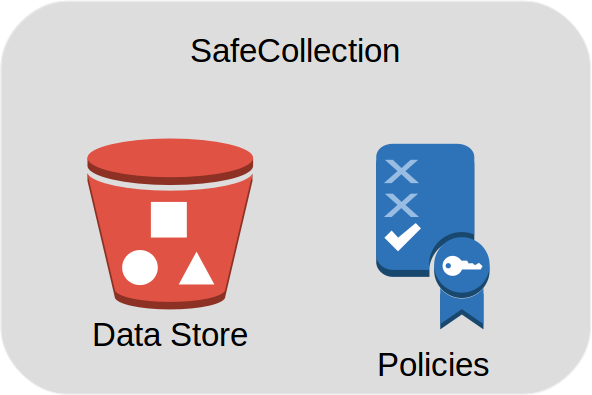
\includegraphics[width=0.45\textwidth]{figures/safecollection.png}
  \caption{Safe collection schema}
  \label{fig:safe_schema}
  \vspace{-1.5em}
\end{figure}

\begin{figure}
  \center
  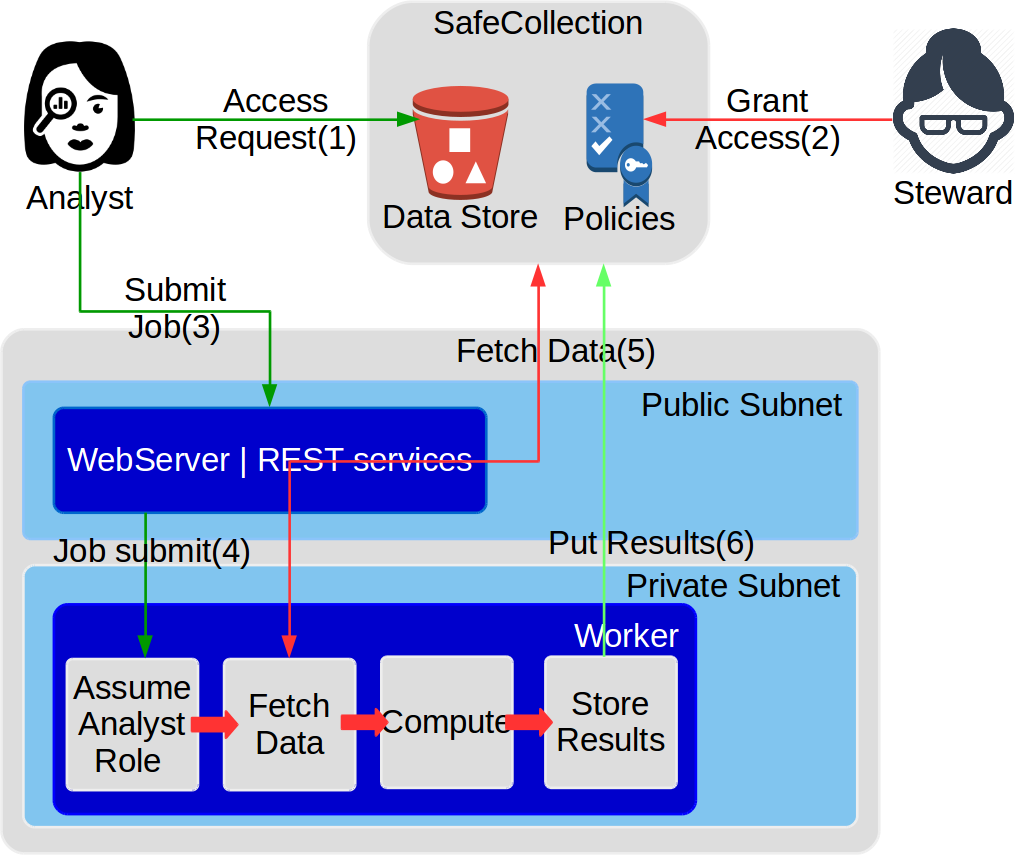
\includegraphics[width=0.45\textwidth]{figures/safe_flow.png}
  \caption{Safe collection schema}
  \label{fig:flow1}
  \vspace{-1.5em}
\end{figure}


\begin{figure}
  \center
  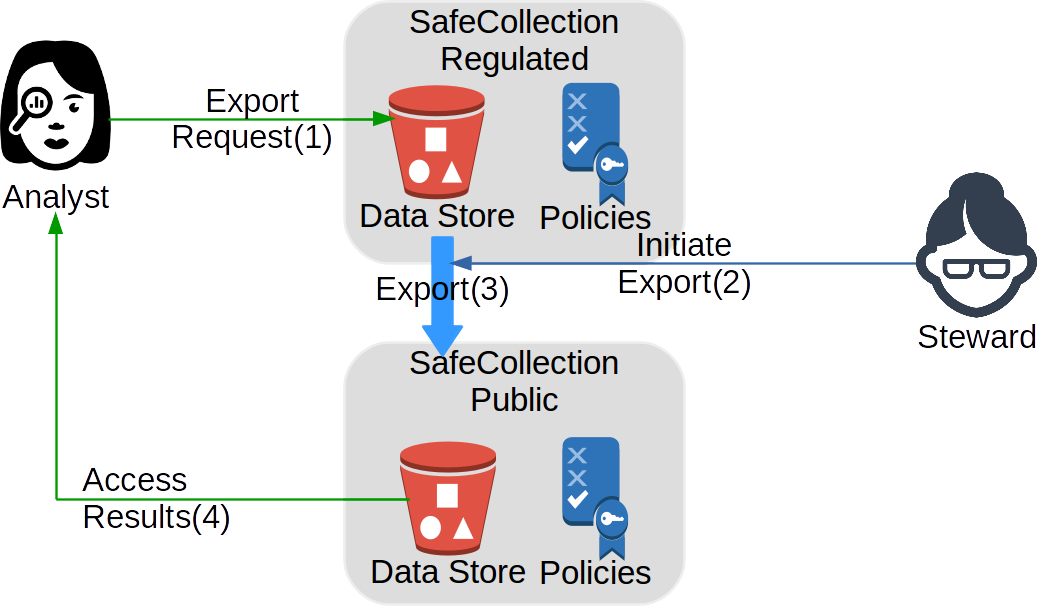
\includegraphics[width=0.45\textwidth]{figures/export_flow.png}
  \caption{Safe collection schema}
  \label{fig:flow2}
  \vspace{-1.5em}
\end{figure}









